%=============================================================================
% FloodEye -- AWS Production Scaling & Cost Plan (USD & INR Pricing)
% Compile: pdflatex aws_cost_plan.tex (run twice for cross-references)
%=============================================================================
\documentclass[11pt,a4paper]{article}

\usepackage[T1]{fontenc}
\usepackage[utf8]{inputenc}
\usepackage{lmodern}
\usepackage[top=2.2cm,bottom=2.2cm,left=2.5cm,right=2.5cm]{geometry}
\linespread{1.12}
\usepackage{amsmath}
\usepackage{graphicx}
\usepackage[dvipsnames]{xcolor}
\usepackage{float}
\usepackage{booktabs}
\usepackage{tabularx}
\usepackage{enumitem}
\usepackage{fancyhdr}
\usepackage{titlesec}
\usepackage{tikz}
\usetikzlibrary{shapes.geometric,arrows.meta,positioning}
\usepackage[colorlinks=true,linkcolor=blue,urlcolor=blue]{hyperref}

%--- Colours ---
\definecolor{FloodBlue}{HTML}{1D4ED8}
\definecolor{FloodGray}{HTML}{475569}
\definecolor{AWSOrg}{HTML}{FF9900}
\definecolor{HeaderBg}{HTML}{1D4ED8}

%--- Section headings ---
\titleformat{\section}{\normalfont\Large\bfseries\color{FloodBlue}}{\thesection}{1em}{}
\titleformat{\subsection}{\normalfont\large\bfseries\color{FloodGray}}{\thesubsection}{1em}{}
\titleformat{\subsubsection}{\normalfont\normalsize\bfseries\color{FloodGray}}{\thesubsubsection}{1em}{}
\titlespacing*{\section}{0pt}{14pt}{6pt}
\titlespacing*{\subsection}{0pt}{10pt}{4pt}
\titlespacing*{\subsubsection}{0pt}{8pt}{2pt}

%--- Header / footer ---
\setlength{\headheight}{14pt}
\pagestyle{fancy}
\fancyhf{}
\fancyhead[L]{\small\textit{FloodEye -- AWS Production Scaling \& Cost Plan (USD/INR)}}
\fancyhead[R]{\small\thepage}
\fancyfoot[C]{\small\textcolor{FloodGray}{Technology Innovation Hub (TIH), IIT Guwahati}}
\renewcommand{\headrulewidth}{0.4pt}
\renewcommand{\footrulewidth}{0.4pt}

\newcommand{\colorrule}{\vspace{4pt}\noindent\textcolor{FloodBlue!30}{\rule{\linewidth}{0.5pt}}\vspace{6pt}}

%--- TikZ styles ---
\tikzset{
  aws/.style={rectangle,rounded corners=4pt,draw=AWSOrg,fill=AWSOrg!12,
              text width=2.6cm,minimum height=0.85cm,align=center,font=\footnotesize\bfseries},
  iot/.style={rectangle,rounded corners=4pt,draw=FloodBlue,fill=FloodBlue!10,
              text width=2.6cm,minimum height=0.85cm,align=center,font=\footnotesize\bfseries},
  arr/.style={-{Stealth[length=4pt]},thick,color=FloodBlue},
}

%=============================================================================
\begin{document}
%=============================================================================

%--- Compact Header / Title Block ---
\begin{center}
  {\color{AWSOrg}\rule{\linewidth}{2.5pt}}\par\vspace{4pt}
  {\Huge\bfseries\color{FloodBlue}FloodEye\par}
  \vspace{4pt}
  {\LARGE\bfseries\color{FloodGray}AWS Production Scaling \& Infrastructure Cost Plan\par}
  \vspace{4pt}
  {\large\textbf{Dual Currency Analysis: USD (\$) \& INR (INR~@~84.50/\$)}}\par
  \vspace{6pt}
  {\small\textit{Technology Innovation Hub (TIH), IIT Guwahati \quad|\quad July 2025 \quad|\quad Region: AWS ap-south-1 (Mumbai)}}\par
  \vspace{2pt}
  {\color{FloodBlue}\rule{\linewidth}{1pt}}
\end{center}

\vspace{-4pt}
%=============================================================================
\section{Executive Summary}
%=============================================================================

This document outlines the production-ready infrastructure roadmap and dual-currency cost model (\textbf{USD} and \textbf{INR}) for transitioning the \textbf{FloodEye} IoT flood monitoring platform from a prototype to an enterprise-grade disaster warning system on AWS. The current prototype relies on HTTP polling via ThingSpeak and client-side inference. To support high-concurrency monsoon alerts across Assam and Northeast India, five core enhancement pillars are mapped to managed AWS services:

\begin{enumerate}[leftmargin=1.8em,label=\textbf{\arabic*.},itemsep=1pt,topsep=2pt]
  \item \textbf{MQTT Protocol:} Migrating to mutual TLS MQTT ingestion via \textbf{AWS IoT Core}.
  \item \textbf{PostgreSQL Database:} Replacing JSON files with \textbf{Amazon RDS for PostgreSQL} + \textbf{TimescaleDB}.
  \item \textbf{Multi-Node Mesh Architecture:} Distributed containerized API execution on \textbf{AWS ECS Fargate} + ALB.
  \item \textbf{SMS/WhatsApp Gateway:} TRAI-compliant emergency alerting via \textbf{Amazon SNS}, \textbf{Lambda}, and \textbf{Twilio}.
  \item \textbf{Advanced ML Inference:} Server-side multi-horizon TFT forecasting on \textbf{Amazon SageMaker Serverless}.
\end{enumerate}

All cost estimates assume a baseline \textbf{50-node regional deployment} transmitting every 15 seconds ($\approx$\textbf{8.64 million telemetry messages/month}) in \textbf{AWS ap-south-1 (Mumbai)}, benchmarked at an exchange rate of \textbf{\$1 USD = INR~84.50}.

\colorrule

%=============================================================================
\section{AWS Service Architecture}
%=============================================================================

\subsection{Architecture Diagram}

\begin{figure}[htbp]
\centering
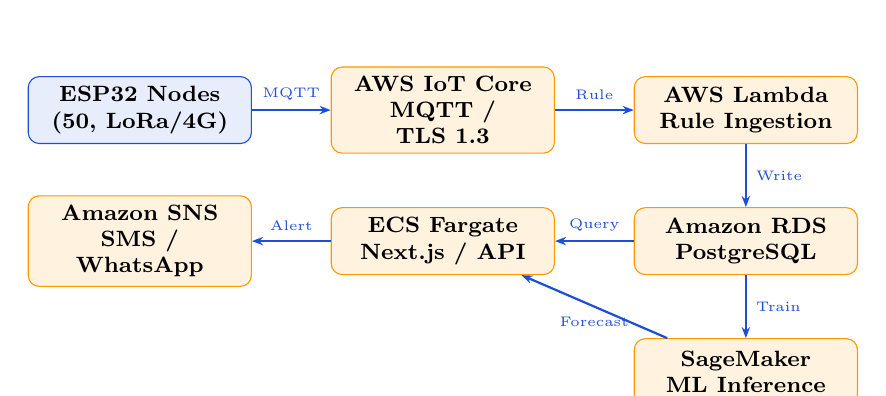
\begin{tikzpicture}[node distance=1.1cm and 0.8cm]
  \node[iot] (esp)    {ESP32 Nodes\\(50, LoRa/4G)};
  \node[aws, right=1.0cm of esp] (iot)    {AWS IoT Core\\MQTT / TLS 1.3};
  \node[aws, right=1.0cm of iot] (lam)    {AWS Lambda\\Rule Ingestion};
  \node[aws, below=0.8cm of lam] (rds)    {Amazon RDS\\PostgreSQL};
  \node[aws, left=1.0cm  of rds] (ecs)    {ECS Fargate\\Next.js / API};
  \node[aws, below=0.8cm of rds] (sage)   {SageMaker\\ML Inference};
  \node[aws, left=1.0cm  of ecs] (sns)    {Amazon SNS\\SMS / WhatsApp};

  \draw[arr] (esp)  -- node[above,font=\tiny]{MQTT} (iot);
  \draw[arr] (iot)  -- node[above,font=\tiny]{Rule}  (lam);
  \draw[arr] (lam)  -- node[right,font=\tiny]{Write} (rds);
  \draw[arr] (rds)  -- node[above,font=\tiny]{Query} (ecs);
  \draw[arr] (rds)  -- node[right,font=\tiny]{Train} (sage);
  \draw[arr] (sage) -- node[below,font=\tiny]{Forecast} (ecs);
  \draw[arr] (ecs)  -- node[above,font=\tiny]{Alert} (sns);
\end{tikzpicture}
\caption{FloodEye Production Cloud Architecture on AWS ap-south-1 (Mumbai)}
\label{fig:aws-arch}
\end{figure}

\subsection{Pillar-by-Pillar Technical Specifications}

\begin{itemize}[leftmargin=1.5em,itemsep=3pt,topsep=2pt]
  \item \textbf{Pillar 1 -- MQTT (AWS IoT Core):} Replaces HTTP polling with lightweight MQTT over TLS (Port 8883) using X.509 client certificates per node. Handles $50 \times 4\,\text{msg/min} \times 43{,}200\,\text{min/mo} = \mathbf{8.64\,M}$ messages/month with QoS 1 reliability.
  \item \textbf{Pillar 2 -- PostgreSQL (Amazon RDS + TimescaleDB):} Managed \texttt{db.t4g.small} instance (2 vCPU, 2 GB RAM, 50 GB gp3 SSD) running PostgreSQL with the TimescaleDB hypertable extension for high-speed time-series queries and 7-day automated backups.
  \item \textbf{Pillar 3 -- Multi-Node App (ECS Fargate + CloudFront):} Containerized Next.js frontend and API running across 2 Fargate tasks (0.5 vCPU, 1 GB RAM each) behind an Application Load Balancer. CloudFront CDN caches static assets, reducing network egress by 80\%.
  \item \textbf{Pillar 4 -- SMS Alert Gateway (SNS + Lambda + Twilio):} Event-driven threshold breaches invoke AWS Lambda to broadcast TRAI-compliant SMS and WhatsApp alerts. ElastiCache Redis (\texttt{t4g.micro}) deduplicates alerts within a 15-minute sliding window.
  \item \textbf{Pillar 5 -- ML Forecasting (SageMaker Serverless):} Replaces browser-side CNN/LSTM with a Temporal Fusion Transformer (TFT) deployed on SageMaker Serverless Inference (pay-per-request), delivering 1h, 4h, and 12h river flood stage forecasts.
\end{itemize}

\colorrule

%=============================================================================
\section{Monthly Infrastructure Cost Plan (USD \& INR)}
%=============================================================================

Table~\ref{tab:cost} presents the itemized monthly expenditure for a \textbf{50-node pilot deployment} in AWS ap-south-1 (Mumbai), showing both USD (\$) and INR amounts (\textbf{INR~84.50 / USD}). The table is formatted to fit cleanly within standard page margins.

\begin{table}[htbp]
\centering
\renewcommand{\arraystretch}{1.2}
\footnotesize
\begin{tabularx}{\linewidth}{l l X r r r}
\toprule
\textbf{Pillar} & \textbf{AWS Service} & \textbf{Specification} & \textbf{Unit (\$)} & \textbf{USD/mo} & \textbf{INR/mo} \\
\midrule
MQTT Protocol   & AWS IoT Core         & 8.64M msgs/month        & \$1.00 / M     & \$10.00  & 845 \\
PostgreSQL      & RDS db.t4g.small     & 2 vCPU, 2 GB, 50 GB SSD & On-Demand      & \$34.00  & 2,873 \\
Multi-Node App  & ECS Fargate + ALB    & 2 tasks, 0.5 vCPU each  & Per-vCPU/hr    & \$28.00  & 2,366 \\
SMS Gateway     & SNS + Lambda + Twilio & 5k SMS + 100K invokes  & \$0.005 / SMS  & \$25.00  & 2,113 \\
ML Inference    & SageMaker Serverless & 100K reqs, 2 GB mem     & Per-invoke     & \$15.00  & 1,268 \\
CDN / Network   & CloudFront + Route53 & 100 GB out, 1M WAF req  & \$0.085 / GB   & \$12.00  & 1,014 \\
Cache Layer     & ElastiCache Redis    & t4g.micro (0.5 GB RAM)  & On-Demand      & \$12.00  & 1,014 \\
Monitoring      & CloudWatch + X-Ray   & 10 GB logs/month        & \$0.50 / GB    & \$8.00   & 676 \\
\midrule
\multicolumn{4}{l}{\textbf{Total Monthly Cost -- 50-Node Production Pilot}} & \textbf{\$144.00} & \textbf{12,168} \\
\multicolumn{4}{l}{\textbf{Annualized Infrastructure Budget (12 Months)}}   & \textbf{\$1,728.00} & \textbf{1,46,016} \\
\bottomrule
\end{tabularx}
\caption{Itemized Monthly AWS Infrastructure Budget (ap-south-1 Mumbai, July 2025)}
\label{tab:cost}
\end{table}

\subsection{Multi-Tier Scaling Projections (50 to 2,000 Nodes)}

Table~\ref{tab:scaling} demonstrates economies of scale as FloodEye expands from a regional pilot to state-wide and national deployment tiers across India.

\begin{table}[htbp]
\centering
\renewcommand{\arraystretch}{1.2}
\footnotesize
\begin{tabularx}{\linewidth}{l c c X r r}
\toprule
\textbf{Deployment Tier} & \textbf{Nodes} & \textbf{Msgs/mo} & \textbf{Database Sizing} & \textbf{USD/mo} & \textbf{INR/mo} \\
\midrule
Pilot (River Basin)     &    50 &   8.64M & db.t4g.small (2 vCPU, 2 GB)   & \$144   & 12,168 \\
District (Kamrup)       &   200 &  34.56M & db.t4g.medium (2 vCPU, 4 GB)  & \$380   & 32,110 \\
State-Wide (Assam)      &   500 &  86.40M & db.r7g.large (2 vCPU, 16 GB)  & \$920   & 77,740 \\
National Grid (India)   & 2,000 & 345.60M & db.r7g.xlarge + Read Replicas & \$3,200 & 2,70,400 \\
\bottomrule
\end{tabularx}
\caption{Infrastructure Cost Projections by Deployment Tier (USD \& INR)}
\label{tab:scaling}
\end{table}

\colorrule

%=============================================================================
\section{Cost Optimisation Strategies}
%=============================================================================

By implementing AWS well-architected cost optimization techniques, the effective operational cost of the 50-node pilot can be reduced by \textbf{30--40\%}:

\begin{enumerate}[leftmargin=1.8em,label=\textbf{\arabic*.},itemsep=2pt,topsep=2pt]
  \item \textbf{RDS Reserved Instances (1-Year Term):} Committing to a 1-year No-Upfront Reserved Instance for PostgreSQL reduces database compute costs by $\approx$35\%, saving \textbf{\$12/month (INR~1,014/month)}.
  \item \textbf{MQTT Payload Compression (CBOR):} Encoding ESP32 telemetry payloads in Concise Binary Object Representation (CBOR) instead of verbose JSON reduces MQTT byte volume by 50\%, cutting network ingestion overhead.
  \item \textbf{Seasonal SageMaker Scaling:} Monsoon season in Assam spans May to September. During dry winter months, SageMaker Serverless concurrency limits can be scaled to zero, saving \textbf{\$15/month (INR~1,268/month)} in idle inference fees.
  \item \textbf{S3 Glacier Tiered Storage:} Telemetry records older than 90 days are automatically migrated from RDS gp3 SSD (\$0.115/GB) to Amazon S3 Glacier Flexible Retrieval (\$0.004/GB), cutting historical data archiving costs by \textbf{96\%}.
  \item \textbf{EC2 Spot Instances for Retraining:} Running weekly Temporal Fusion Transformer model retraining jobs on EC2 Spot Instances saves up to \textbf{70\%} compared to On-Demand GPU instances.
  \item \textbf{CloudFront Edge Caching:} Caching frontend UI bundles and static GeoJSON flood maps at CloudFront edge locations reduces Fargate data transfer out by 80\%, saving \textbf{\$9/month (INR~760/month)}.
\end{enumerate}

\noindent
\textbf{Optimized Pilot Cost:} Applying these six strategies reduces the 50-node monthly expenditure from \textbf{\$144 (INR~12,168)} down to approximately \textbf{\$95/month (INR~8,028/month)}, or an annualized budget of \textbf{INR~96,336/year}.

\colorrule

%=============================================================================
\section{Phased 6-Month Implementation Roadmap}
%=============================================================================

\begin{table}[htbp]
\centering
\renewcommand{\arraystretch}{1.2}
\footnotesize
\begin{tabularx}{\linewidth}{c l X r}
\toprule
\textbf{Phase} & \textbf{Enhancement Pillar} & \textbf{Key AWS Managed Services} & \textbf{Timeline} \\
\midrule
1 & PostgreSQL Database Migration & Amazon RDS for PostgreSQL, Prisma ORM  & Month 1    \\
2 & MQTT Mutual TLS Ingestion     & AWS IoT Core, X.509 Certs, IoT Rules   & Month 2    \\
3 & Multi-Node Dashboard Mesh     & AWS ECS Fargate, ALB, CloudFront CDN   & Month 3    \\
4 & SMS/WhatsApp Alert Gateway    & Amazon SNS, AWS Lambda, Twilio / MSG91 & Month 4    \\
5 & Server-side TFT ML Model      & Amazon SageMaker, EventBridge, S3      & Month 5--6 \\
\bottomrule
\end{tabularx}
\caption{Phased Production Rollout Roadmap (Months 1 to 6)}
\label{tab:roadmap}
\end{table}

%=============================================================================
\section{Summary}
%=============================================================================

The \textbf{FloodEye} platform can transition from an HTTP-based single-node prototype to a fault-tolerant, 50-node production flood monitoring network on AWS ap-south-1 for an unoptimized monthly budget of \textbf{\$144.00 (INR~12,168)} and an optimized budget of \textbf{\$95.00 (INR~8,028)}. This architecture guarantees sub-second MQTT telemetry, resilient time-series storage, automated multi-channel emergency broadcasting, and continuous machine learning flood stage forecasting.

\vspace{10pt}
\begin{center}
  {\color{AWSOrg}\rule{0.35\linewidth}{1.5pt}}
  \quad
  {\color{FloodBlue}\rule{0.35\linewidth}{1.5pt}}
\end{center}

\end{document}
